
\section{Filtro con GIC}

A continuaci\'on se estudia la implementaci\'on de un filtro mediante el circuito de la figura \ref{circ1}. Si bien una parte del circuito parecer\'ia ser un GIC, debido a la resistencia R8 no lo es.

\begin{figure}[H] %!ht
	\centering
	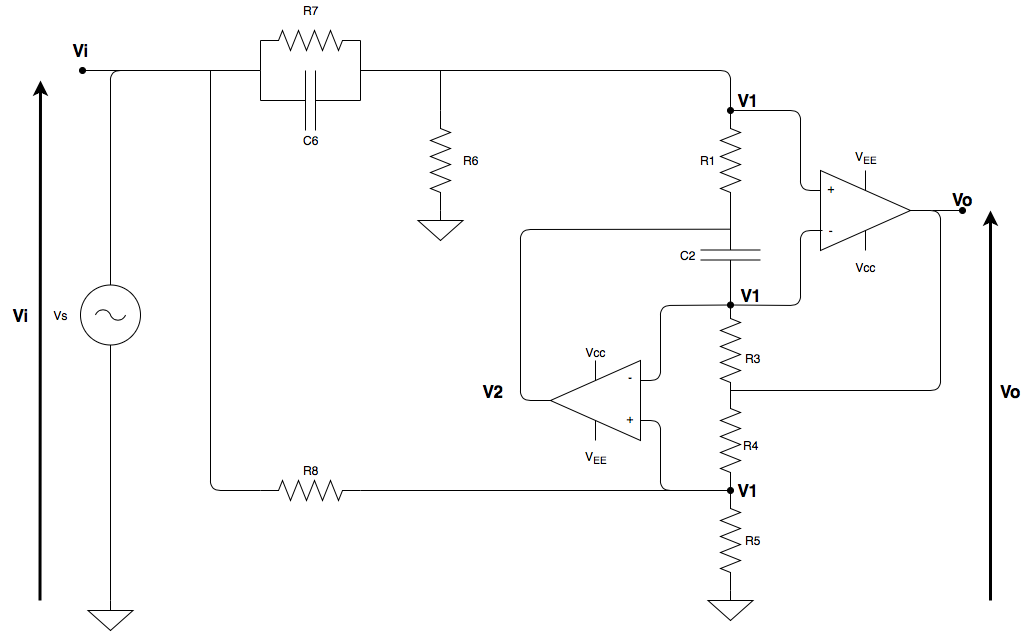
\includegraphics[scale=0.4]{../EJ1/circuito1.png}
	%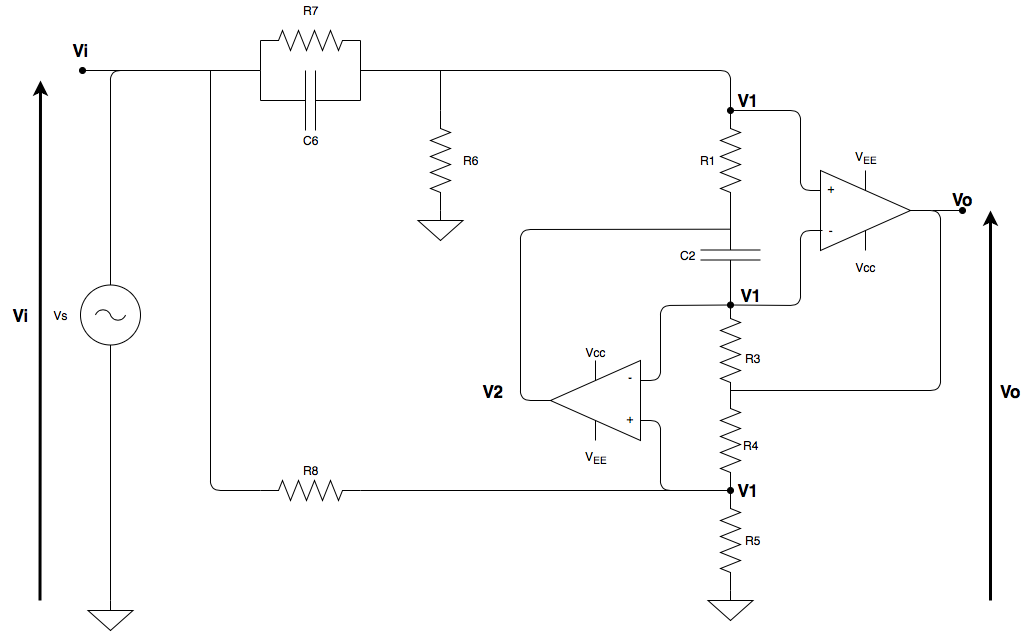
\includegraphics[width=10cm,height=10cm,keepaspectratio]{../EJ1/circuito1.png}
	\caption{Circuito empleado como filtro, involucrando una configuraci\'on similar a un GIC.}
	\label{circ1}
\end{figure}


\subsection{Funci\'on transferencia del circuito}
Debido a la complejidad del circuito \ref{circ1}, se  calcul\'o $\frac{V_O}{V_I}$ considerando a los dos amplificadores operacionales como ideales. Esto implica que se haya considerado $A_{vol}$ infinito. Para este an\'alisis, mediante resoluci\'on por nodos, se parti\'o de las relaciones entre corrientes entranes y salientes a cada uno de los tres nodos indicados en el circuito con tensi\'on $V_1$:

\begin{equation}
	\begin{cases}
		\frac{V_i - V_1}{(R_7 // \frac{1}{sC_6})} = \frac{V_1}{R_6} + \frac{V_1 - V_2}{R_1}\\ \\
		\frac{V_2 - V_1}{\frac{1}{sC_2}} = \frac{V_1 - V_O}{R_3}\\ \\
		\frac{V_O - V_1}{R_4} = \frac{V_1 - V_i}{R_8} + \frac{V_1}{R_5}
	\end{cases}
	\label{ecsbase}
\end{equation}

Operando algebraicamente, a partir de las ecuaciones \ref{ecsbase} se obtiene la funci\'on transferencia del circuito \ref{circ1}. Siendo $s = j\omega$, la misma se muestra a continuaci\'on:

\begin{equation}
 	H(s) = \frac{V_O}{V_I} = \frac{R_4 + R_5}{R_5} \cdot 
 	\frac
 	{ s^2
 		+\frac{R_4 R_6 R_8 + R_5 R_6 R_8 - R_4 R_5 R_7}{C_6 R_6 R_7 R_8 (R_4 + R_5)} \cdot s
 		+\frac{R_4 R_5}{C_2 C_6 R_1 R_3 R_8 (R_4 + R_5)}}
 	{s^2
 		+\frac{R_6 + R_7}{C_6 R_6 R_7} \cdot s
 		+\frac{R_4 (R_5 + R_8)}{C_2 C_6 R_1 R_3 R_5 R_8}
 	}
	\label{vovi}
\end{equation}


\subsubsection{Caracter\'sticas del circuito a partir de la funci\'on transferencia}

Si bien observando la funci\'on transferencia se puede decir que se trata de un filtro de segundo orden, a continuaci\'on se analiza m\'as en detalle a qu\'e tipo de filtro corresponde.

\paragraph*{Polos y ceros:}
A partir del t\'ermino de grado cero del numerador y del denominador del cociente de polinomios de la expresi\'on de $H(s)$ (Ecuaci\'on \ref{vovi}) se puede obtener la expresi\'on de los polos y ceros del circuito, ya que simb\'olicamente dichos t\'erminos son $\left(\frac{s}{\omega_Z}\right)^2$ y $\left(\frac{s}{\omega_P}\right)^2$respectivamente. Por lo tanto,

\begin{equation}
	\omega_Z = \pm\sqrt{\frac{R_4 R_5}{C_2 C_6 R_1 R_3 R_8 (R_4 + R_5)}}
	\label{ec_z}
\end{equation}

\begin{equation}
	\omega_P = \pm \sqrt{\frac{R_4 (R_5 + R_8)}{C_2 C_6 R_1 R_3 R_5 R_8}}
	\label{ec_p}
\end{equation}

Observando las diferencias entre los numeradores de las expresiones \ref{ec_z} y \ref{ec_p} se puede ver que como $R_5 < R_5 + 5_8$, el numerador del $\omega_Z$ es menor que el de $\omega_P$. Analizando los denominadores de igual manera, se v\'e que el denominador de $\omega_Z$ es mayor al denominador de $\omega_P$ ya que $R_4 + R_5 > R_5$. Por lo tanto, $\omega_Z < \omega_P$. Esto indica que el circuito \ref{circ1} es un filtro $High-Pass$ $ Notch$.


\paragraph*{Ganancia del circuito (G):}  La ganancia $G$ para el caso de un filtro $High-Pass$ $ Notch$ se obtiene como $\lim_{s\to\infty}H(s)$, estando $H(S)$ definida por la expresi\'on \ref{vovi} y as\'i es como resulta:
 \begin{equation}
	G = \lim_{s\to\infty}H(s) = 1 + \frac{R_4}{R_5} 
\label{G}
\end{equation}

\paragraph*{Factor de calidad (Q):} El coeficinete que acompa\~na a "s" en el denominador de la expresi\'on \ref{vovi} es $\frac{\omega_P}{Q}$. Por lo tanto, a partir de dicho coeficiente y de la expresi'on \ref{ec_p} correspondiente al $\omega_P$, se obtiene que:

\begin{equation}
	Q = \frac{R_{6} R_{7}}{R_{6} + R_{7}} \cdot \sqrt{\frac{C_{6} R_{4} \left(R_{5} + R_{8}\right)}{C_{2} R_{1} R_{3}R_{5} R_{8} }}
\end{equation}
	
	
	
	
	
	
\subsection{An\'alisis de sensibilidades}

Para dicho an\'alisis se prosigui\'o mediante la ecuaci\'on \ref{sens}, siendo $X$ el valor de un componente e $Y$ el par\'ametro del circuito cuya sensibilidad respecto a $X$ se quiere calcular.

\begin{equation}
S^{Y}_{X}= \lim_{\Delta X \to \infty} \left(\frac{\Delta Y / Y}{\Delta X / X}\right) = \frac{X}{Y}\cdot\frac{dY}{dX}
\label{sens}
\end{equation}

Los par\'ametros sobre los que se analiz\'o la sensibilidad de cada uno de los componentes son $\omega_Z$, $\omega_P$ y $Q$. Sus resultados fueron los siguientes:

Sensibilidades de $\omega_Z$ respecto a cada componente del circuito:
\begin{equation}
	\begin{cases}
	S^{\omega_Z}_{R_4}= \frac{1}{2} \cdot \frac{R_{5}}{R_{4} + R_{5}}\\ \\
	S^{\omega_Z}_{R_5}= \frac{1}{2} \cdot \frac{R_{4}}{R_{4} + R_{5}}\\ \\
		S^{\omega_Z}_{C_2} = S^{\omega_Z}_{C_6}= S^{\omega_Z}_{R_1}=S^{\omega_Z}_{R_3}=S^{\omega_Z}_{R_8}    =- \frac{1}{2} 
	\end{cases}
\end{equation}

Sensibilidades de $\omega_P$ respecto a cada componente del circuito:
\begin{equation}
\begin{cases}
	S^{\omega_P}_{R_5} =	-  \frac{1}{2} \cdot \frac{R_{8}}{R_{5} + R_{8}} \\ \\
	S^{\omega_P}_{R_8} =	-  \frac{1}{2} \cdot \frac{R_{5}}{R_{5} + R_{8}}\\ \\
	S^{\omega_P}_{C_2} = S^{\omega_P}_{C_6}= S^{\omega_P}_{R_1}=S^{\omega_P}_{R_3}=	-  \frac{1}{2}\\ \\
	S^{\omega_P}_{R_4} = \frac{1}{2}
	\end{cases}
\end{equation}

Sensibilidades de $Q$ respecto a cada componente del circuito:
\begin{equation}
\begin{cases}
S^{Q}_{R_6} = \frac{R_{7}}{R_{6} + R_{7}}\\ \\
S^{Q}_{R_7} = \frac{R_{6}}{R_{6} + R_{7}}\\ \\
S^{Q}_{R_5} = \frac{1}{2} \frac{(C_{2} R_{1} R_{3} R_{5} R_{8})^2 \left(C_{6} R_{4} R_{5} - 1\right)}{C_{6} R_{4} \left(R_{5} + R_{8}\right) \left(R_{6} + R_{7}\right)^{2}} \\ \\
S^{Q}_{R_8} = \frac{1}{2} \frac{(C_{2} R_{1} R_{3} R_{5} R_{8})^2 \left(C_{6} R_{4} R_{8} - 1\right)}{C_{6} R_{4} \left(R_{5} + R_{8}\right) \left(R_{6} + R_{7}\right)^{2}} \\ \\
S^{Q}_{C_6} = S^{Q}_{R_4} =\frac{1}{2} \\ \\
S^{Q}_{C_2} = S^{Q}_{R_1} = S^{Q}_{R_3} =-\frac{1}{2}
\end{cases}
\end{equation}


\subsection{Dise\~no del circuito - Selecci\'on de componentes}
Para elegir los valores de cada uno de los componentes del circuito, se tuvieron en cuenta las sugerencias indicadas en el enunciado del trabajo pr\'actico.

\begin{itemize}
	\item $R_1 = R_3 = R_8 = R$
	\item $R_6 = (1 + k^2) Q R$
	\item $R_7 = (1 + \frac{1}{k^2})Q R$
	\item $R_4 = \frac{2k^2}{1+k^2}R$
	\item $R_5 = \frac{2k^2}{1-k^2}R$
	\item $C_2 = C_6 = C$
	\item $k = \frac{\omega_Z}{\omega_P} \leqslant 1 $
\end{itemize}

Reemplazando con los valores de las sugerencias previamente mencionadas, se reescribe la funci\'on transferencia de la ecuaci\'on \ref{vovi} para mayor simplicidad:

\begin{equation}
	H(s) = \frac{2}{1+k^2} \cdot \frac{s^2 + \left( \frac{k}{RC}\right)^2}{s^2 + \frac{1}{RCQ} s + \left(\frac{1}{RC}\right)^2}
	\label{vovi_simple}
\end{equation}


La siguiente tabla presenta las especificaciones consideradas para el dise\~no del circuito:

\begin{table}[h!]
	\centering
	\begin{tabular}{c c c}%
		\bfseries $\omega_P$ & Q & $|H(\infty)| (dB)$ \\ \hline
		$13000 \frac{rad}{s}$ & $2$ & $4dB$\\
		\hline
	\end{tabular}
	\caption{Especificaciones de dise\~no}
	\label{especificaciones}
\end{table}

A partir de la ecuaci\'on \ref{vovi_simple} y considerando lo indicado en la tabla \ref{especificaciones}:

\begin{equation}
	\omega_P = \frac{1}{RC} = 13000\frac{rad}{s}
	\label{dwp}
\end{equation}

Eligiendo $C = 100nF$, el valor de R debe ser tal que cumpla con la ecuaci\'on \ref{dwp}. Entonces $R = \frac{1}{13000 * 100 *10^{-9}} \approx 0,769k\Omega.$




\subsection{Polos y ceros}

Anal\'iticamente se obtienen las siguientes expresiones para los polos y ceros del filtro:

\begin{equation}
s_{z1,z2} = - \frac{R_4  R_6  R_8+R_5  R_6  R_8 - R_4 R_5 R_7}{C_6 R_6 R_7 R_8 \cdot (R_4 + R_5)} \pm \sqrt{\left( \frac{R_4 R_6 R_8 + R_4 R_6 R_8 - R_4 R_5 R_7}{C_6 R_6 R_7 R_8 \cdot (R_4 + R_5)}\right)^2- 4 \cdot \frac{R_4 R_5}{C_2 C_6 R_1 R_3 R_8 \cdot (R_4 + R_5)}}
\label{ceros}
\end{equation}

\begin{equation}
s_{p1,p2} = - \frac{R_6 + R_7}{C_6 R_6 R_7} \pm \sqrt{\left( \frac{R_6 + R_7}{C_6 R_6 R_7}\right)^2 - 4 \cdot \frac{R_4(R_5+R_8)}{C_2 C_6 R_1 R_3 R_5 R_8}}
\label{polos}
\end{equation}


A partir de las expresiones anteriores, al reemplazar con los valores de los componentes empleados, se obtiene el siguiente diagrama de polos y ceros del filtro high pass notch, con $Q\approx 2$:

\begin{figure}[H] %!ht
	\centering
	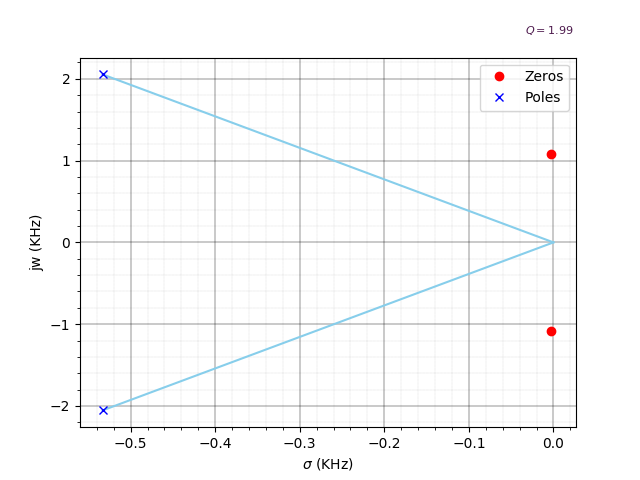
\includegraphics[width=10cm,height=10cm,keepaspectratio]{../EJ1/00GRAFICOS/singularidades.png}
	\caption{Polos y ceros de la funci\'on transferencia del circuito.}
	\label{c1vinmax}
\end{figure}

Los polos se encuentran claramente del lado izquierdo del eje $j\omega$, lo que indica estabilidad del circuito.







%\subsection{Polos y ceros}

\subsection{Variaci\'on de la resistencia $R_8$}

\todo{HACER}

\subsection{Variaci\'on de la resistencia $R_6$}

A continuaci\'on se muestra c\'omo cambian los polos y ceros al modificar la resistencia R6 en la expresi\'on de la transferencia \ref{vovi}, dejando fijas las otras resistencias y los capacitores con los valores determinados para hacer el filtro.


\begin{figure}[H] %!ht
	\centering
	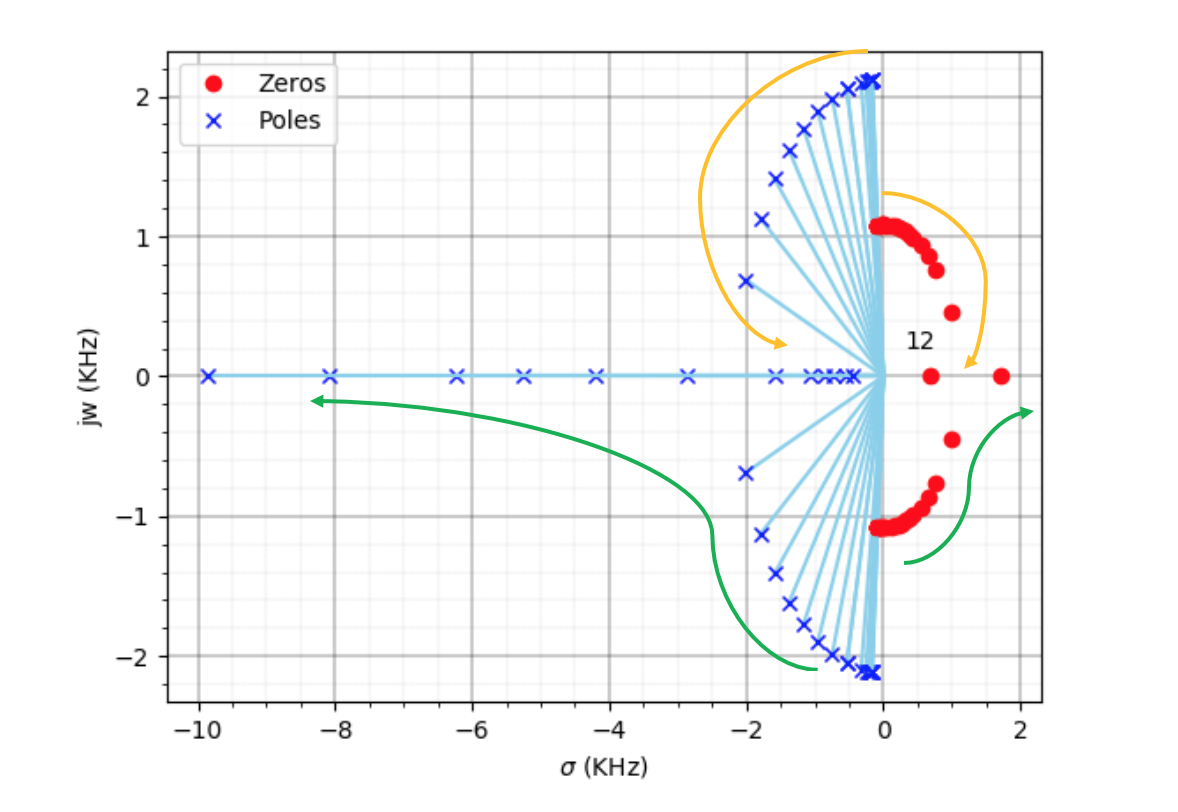
\includegraphics[width=10cm,height=10cm,keepaspectratio]{../EJ1/00GRAFICOS/r6.png}
	\caption{Polos y ceros del circuito al tender R6 a cero}
	\label{r6}
\end{figure}

En la figura \ref{r6} se indica con flechas hacia donde tienden los polos y los ceros al hacer tender R6 a cero. Las flechas amarillas corresponden a la variaci\'on del polo $P1$ y del cero $Z1$ en dicho caso, mientras que las flechas verdes indican el comportamiento del polo $P2$ y del cero $Z2$. Para el caso en el que R6 tiende a infinito, las flechas van en sentido contrario al indicado en la figura. A continuaci\'on se muestran anal\'iticamente dichos comportamientos:

\begin{equation}
	\lim_{R_6\to 0} s_{z1,z2}=  \frac{R_4 R_5}{C_6 R_6 R_8} \pm \frac{R_4 R_5}{C_6 R_6 R_8} \Rightarrow 
	\begin{cases} 
	s_{z1} \to +\infty\\
	s_{z2} \to 0
	\end{cases}
\end{equation}

\begin{equation}
	\lim_{R_6\to 0} s_{p1,p2}=  -\frac{R_6 + R_7}{C_6 R_6 R_7} \pm \frac{R_6 + R_7}{C_6 R_6 R_7} \Rightarrow
	\begin{cases} 
	s_{p1} \to 0\\
	s_{p2} \to -\infty
	\end{cases}
\end{equation}

\begin{equation}
\lim_{R_6\to\infty}s_{z1,z2} =  
\end{equation}

\begin{equation}
\lim_{R_6\to\infty}s_{p1,p2} =  
\end{equation}


\subsection{Limitación de tensi\'on de entrada}

La tensión de entrada máxima del circuito está limitada principalmente por el slew rate slew rate y la saturaci\'on. 

\subsubsection*{Influenccia del slew rate en $V_{in_{max}}$}

Partiendo de:
\begin{equation}
\begin{cases}
SR = m\'ax\bigg\{\frac{ dV_{out}}{dt}\bigg\} \\
V_{in} (f, t) = V_{in_{max}} \cdot sin(2\pi f t) \\
V_{out} (f, t) = \rvert H(f)\rvert \cdot V_{in_{max}} \cdot sin(2 \pi f t)
\end{cases}
\label{srecs}
\end{equation}

Siendo $SR$ el slew rate, $V_{in}$ y $V_{out}$ las se\~nales de entrada y de salida respectivamente y $\rvert H(f)\rvert = V_{out}/V_{in}$ la ganancia del circuito.


\begin{equation}
\frac{dV_{out}}{dt} = \rvert H(f)\rvert V_{in_{max}} 2 \pi f cos(2 \pi f t)
\label{deriv}
\end{equation}

Maximizando la ecuaci\'on \ref{deriv} se obtiene que:

\begin{equation}
SR = m\'ax\bigg\{\frac{dV_{out}}{dt}\bigg\} = \rvert H(f)\rvert 2 \pi f V_{in_{max}} 
\label{max}
\end{equation}

Despejando de la ecuaci\'on \ref{max}:

\begin{equation}
V_{in_{max}}  = \frac{SR}{\rvert H(f)\rvert 2\pi f}
\label{vinmax}
\end{equation}

El valor de SR, para el c\'alculo te\'orico, fue sacado de hojas de datos del amplificador operacional LM833 de Texas Instrument\footnote{Hoja de datos del operacional LM833: https://html.alldatasheet.com/html-pdf/784648/TI1/LM833/52/1/LM833.html}. 
Se encontr\'o que $SR = 7 \frac{V}{\mu s}$. Reemplazando con este valor en la expresi\'on \ref{vin_max}, se obtiene que la tensi\'on de entrada m\'axima limitada por el slew rate es:

\begin{equation}
	V_{in_{max}}  = \frac{\left(17,36 \cdot 10^8 f^{4} - 1.37 \cdot 10^{16} f^{2} + 3.52 \cdot 10^{22}\right)}{f \sqrt{61,19 \cdot 10^5 f^{8} - 62,49 \cdot 10^{12} f^{6} + 2.45 \cdot 10^{20} f^{4} - 3.57 \cdot 10^{26} f^{2} + 1.70 \cdot 10^{32}}}		
\label{vin_max}
\end{equation}


\begin{figure}[H] %!ht
	\centering
	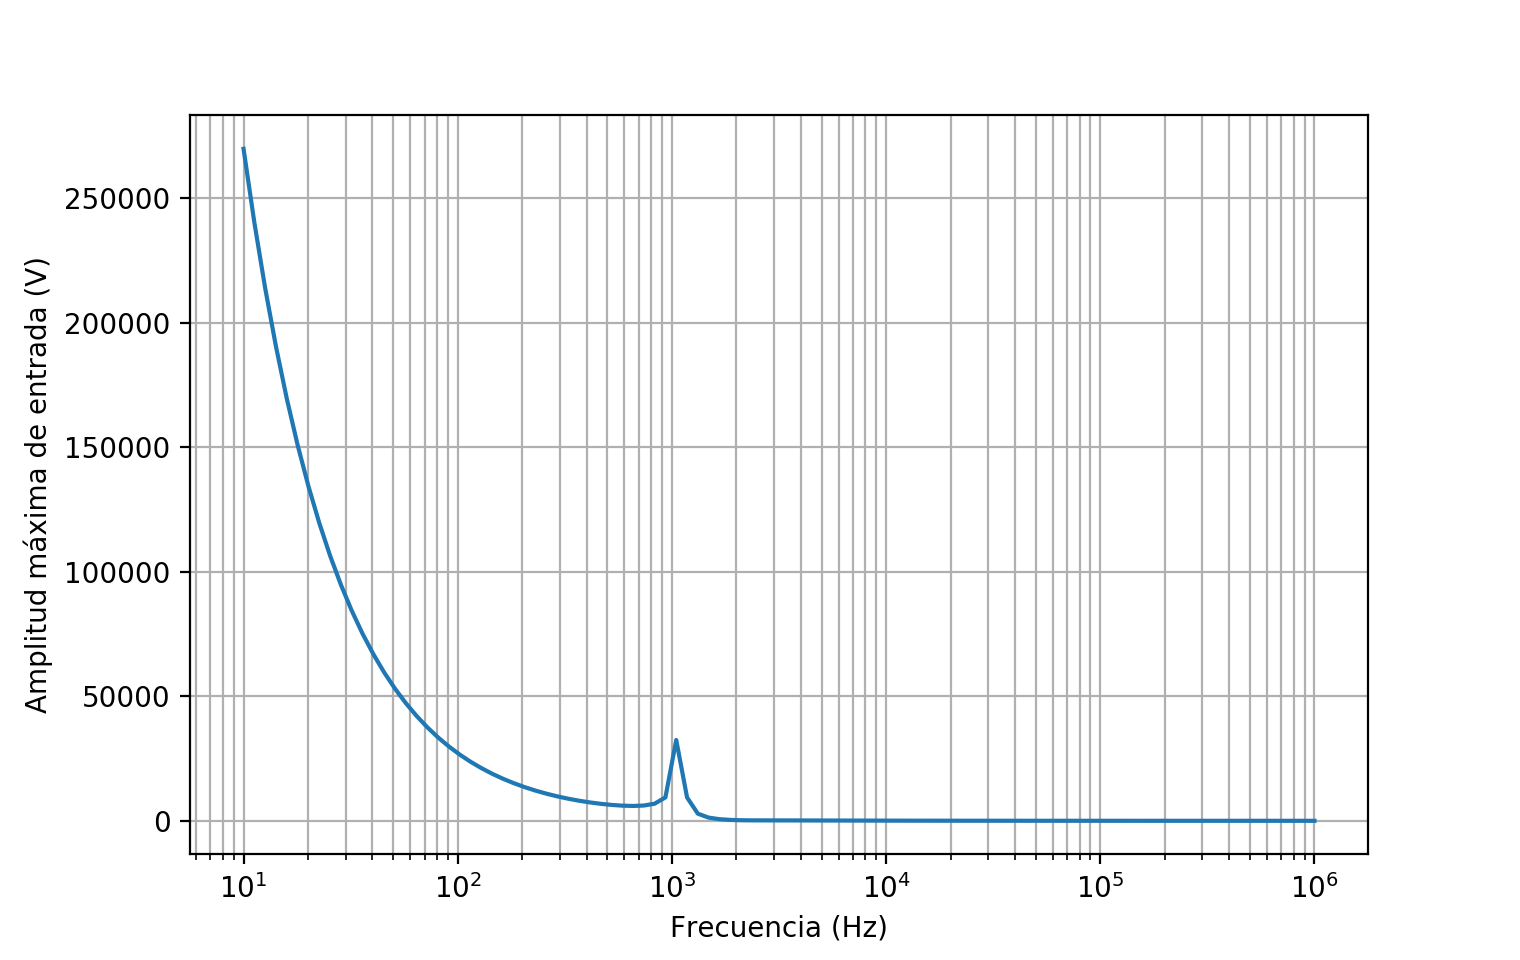
\includegraphics[width=10cm,height=10cm,keepaspectratio]{../EJ1/00GRAFICOS/vinmaxsr.png}
	\caption{Tensi\'on de entrada m\'axima limitada por slew rate.}
	\label{vinmaxsr}
\end{figure}

\subsubsection*{Influenccia de la saturaci\'on en $V_{in_{max}}$}
La tensi\'on pico a pico m\'axima de salida del amplificador operacional es llamada 
tensi\'on de saturasi\'on $V_{sat}$. Te\'oricamente, este valor es igual a $V_{CC}$. Dado que $V_{out} = \rvert H(s) \rvert V_{in}$:

\begin{equation}
V_{in_{max}} = \frac{V_{out_{max}}}{\rvert H(s) \rvert} = \frac{V_{sat}}{\rvert H(s) \rvert} = \frac{V_{CC}}{\rvert H(s) \rvert}
\end{equation}

Dado que en nuestro caso usamos $V_{CC} = \pm15V$, la expresi\'on que se obtiene es:

\begin{equation}
V_{in_{max}} = \frac{15V}{\rvert H(s) \rvert} 
\end{equation}

\todo{en ec anterior poner cuanto da numericamente}

\todo{grafico}
\begin{figure}[H] %!ht
	\centering
	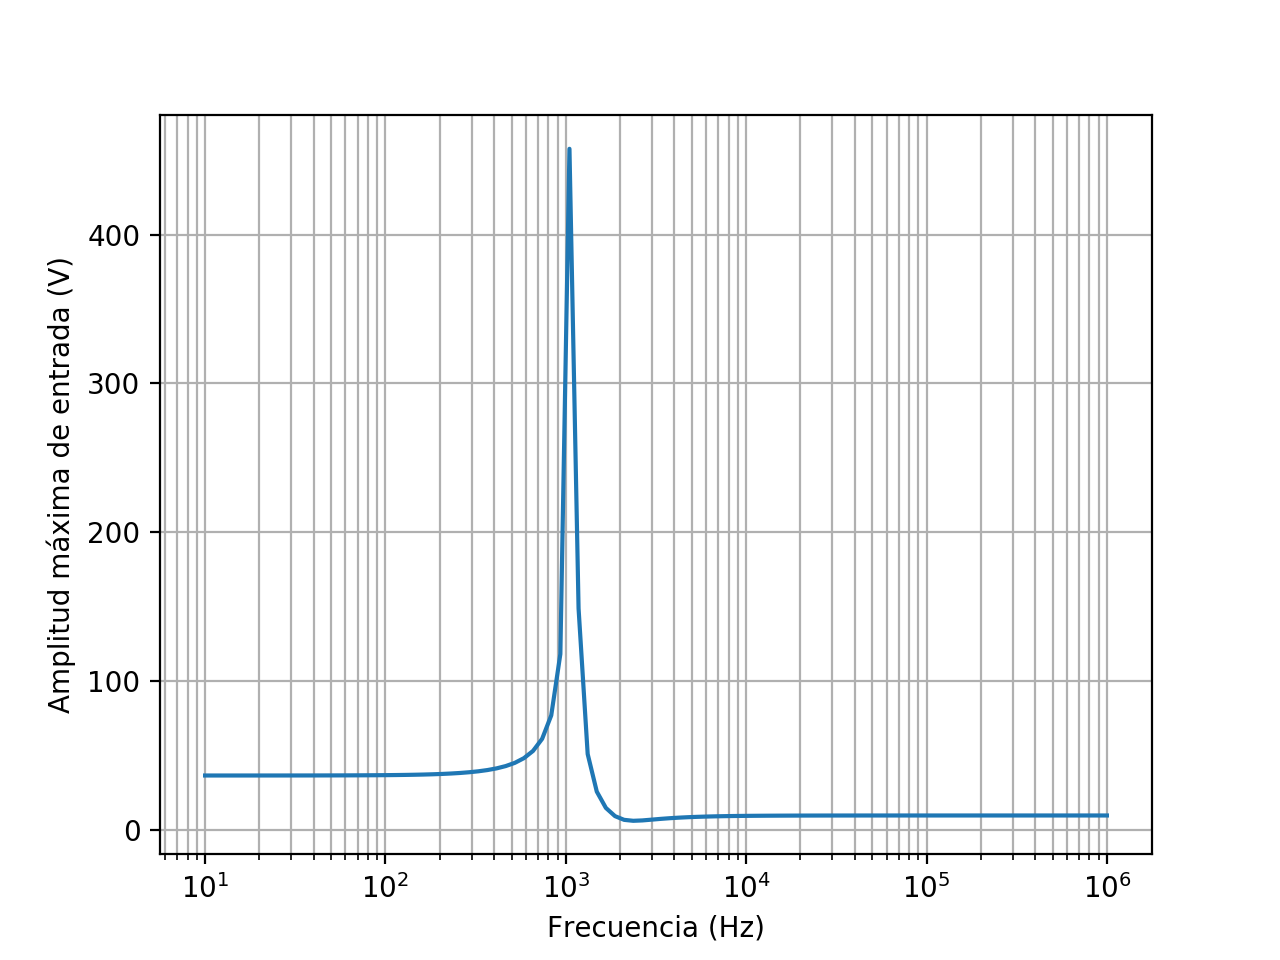
\includegraphics[width=10cm,height=10cm,keepaspectratio]{../EJ1/00GRAFICOS/vinmaxsat.png}
	\caption{Tensi\'on m\'axima de entrada limitada por saturaci\'on.}
	\label{vinmaxsat}
\end{figure}

\subsubsection*{Combinaci\'on del efecto de slew rate y saturaci\'on sobre la tensi\'on m\'axima de entrada}

\todo{grafico}
\begin{figure}[H] %!ht
	\centering
	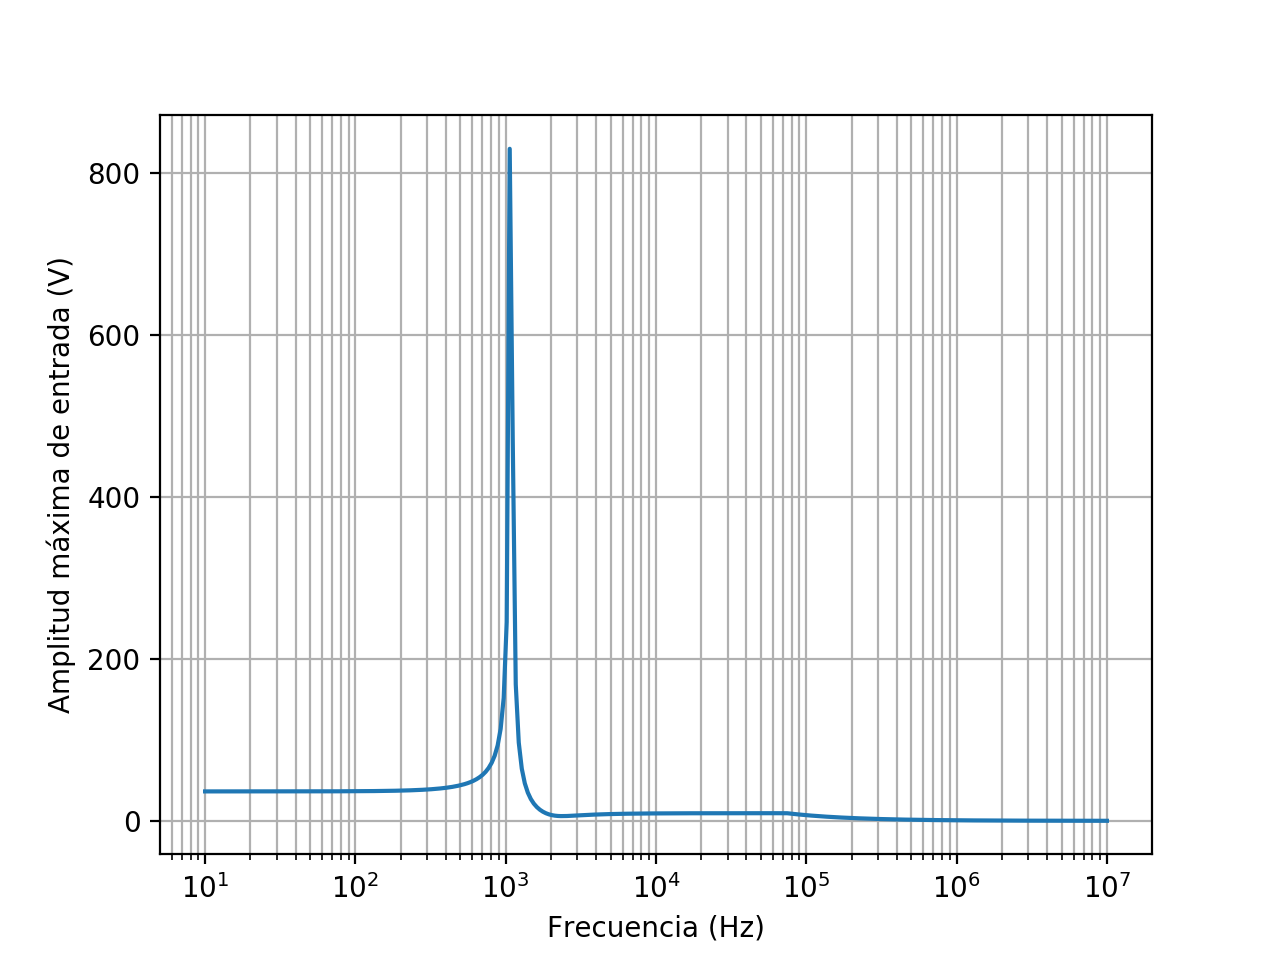
\includegraphics[width=10cm,height=10cm,keepaspectratio]{../EJ1/00GRAFICOS/vinmaxtotal.png}
	\caption{Tensi\'on m\'axima de entrada limitada por slew rate y saturaci\'on.}
	\label{vinmaxtotal}
\end{figure}

\subsection{Transferencia del circuito}

Aqu\'i se compara la funci\'on transferencia del circuito te\'orica, 
medida y simulada mediante el m\'etodo de Montecarlo. Para la medici\'on se emple\'o el bodeador realizado para este trabajo. La simulaci\'on se llev\'o a cabo considerando tolerancias de $1\%$ para las resistencias ya que las empleadas fueron SMD y $10\%$ para los capacitores hole through. Adem\'as, se aclara que la simulaci\'on fue realizada incluyendo las impedancias equivalentes de $10M\Omega // 12pF$ aportadas por las puntas del osciloscopio que se usaron para tomar las mediciones.

\begin{figure}[H] %!ht
	\centering
	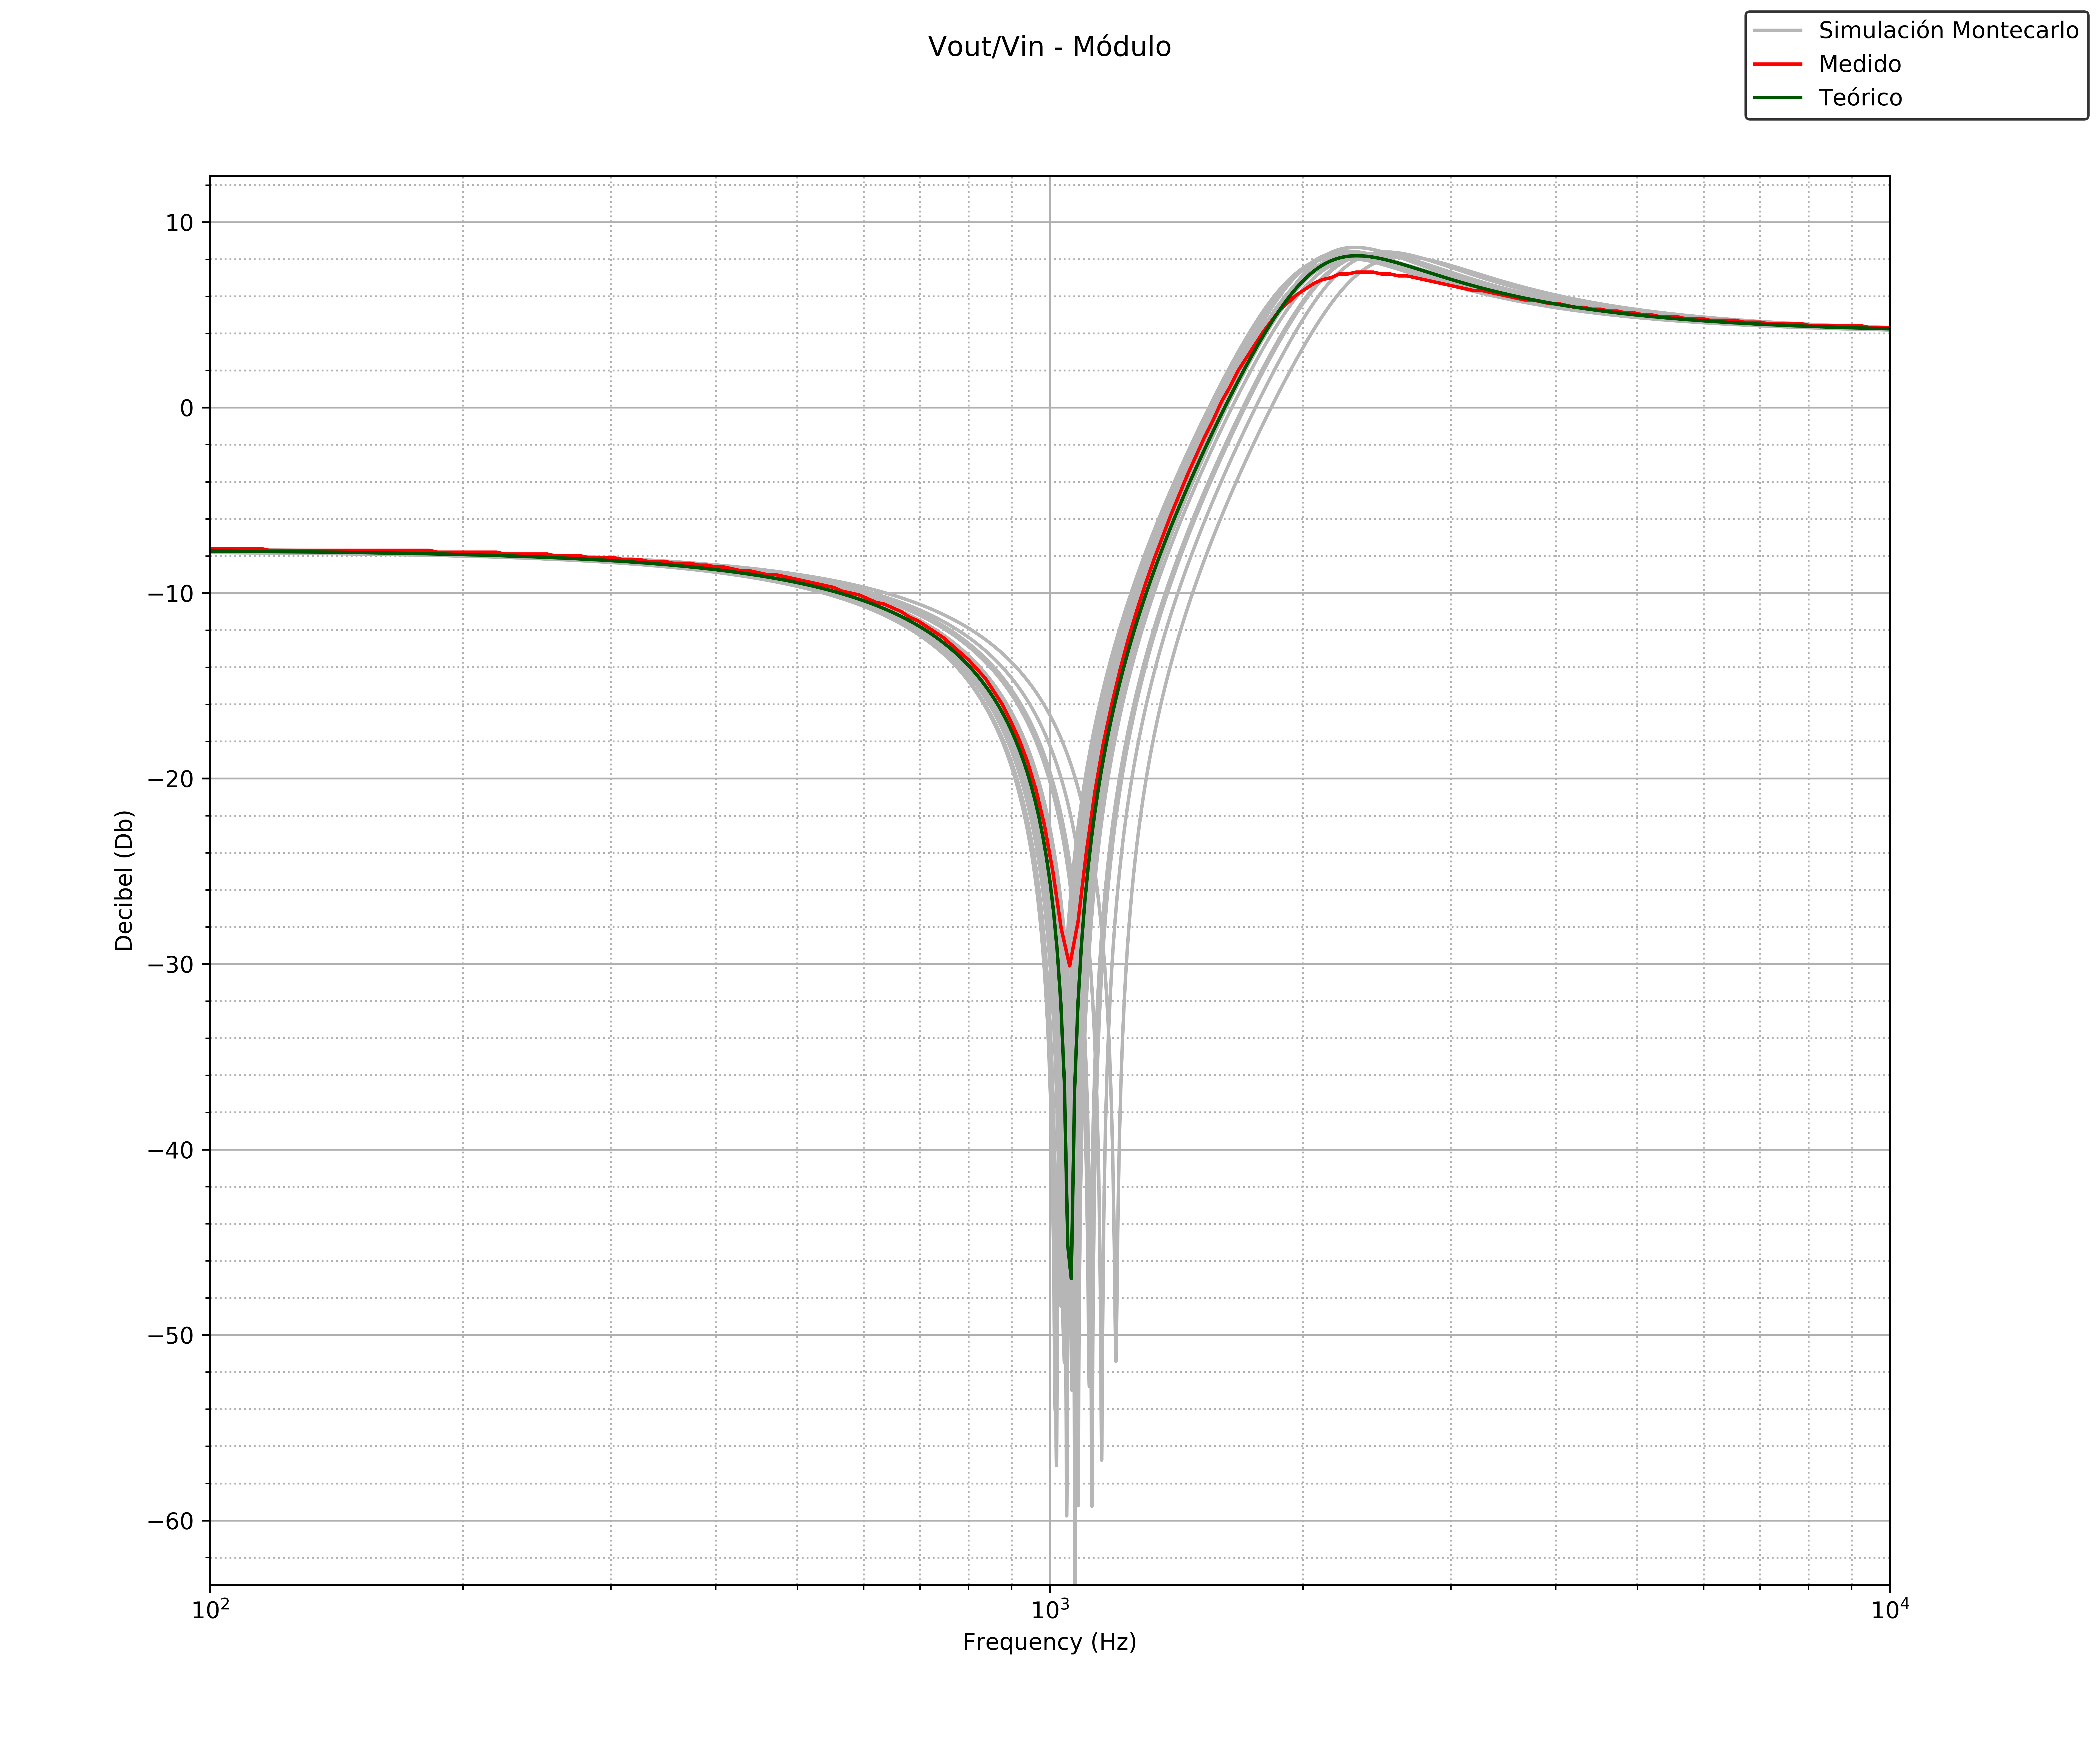
\includegraphics[width=10cm,height=10cm,keepaspectratio]{../EJ1/00GRAFICOS/vovi.png}
	\caption{M\'odulo de la transferencia del circuito.}
	\label{vovi_mod}
\end{figure}

\begin{figure}[H] %!ht
	\centering
	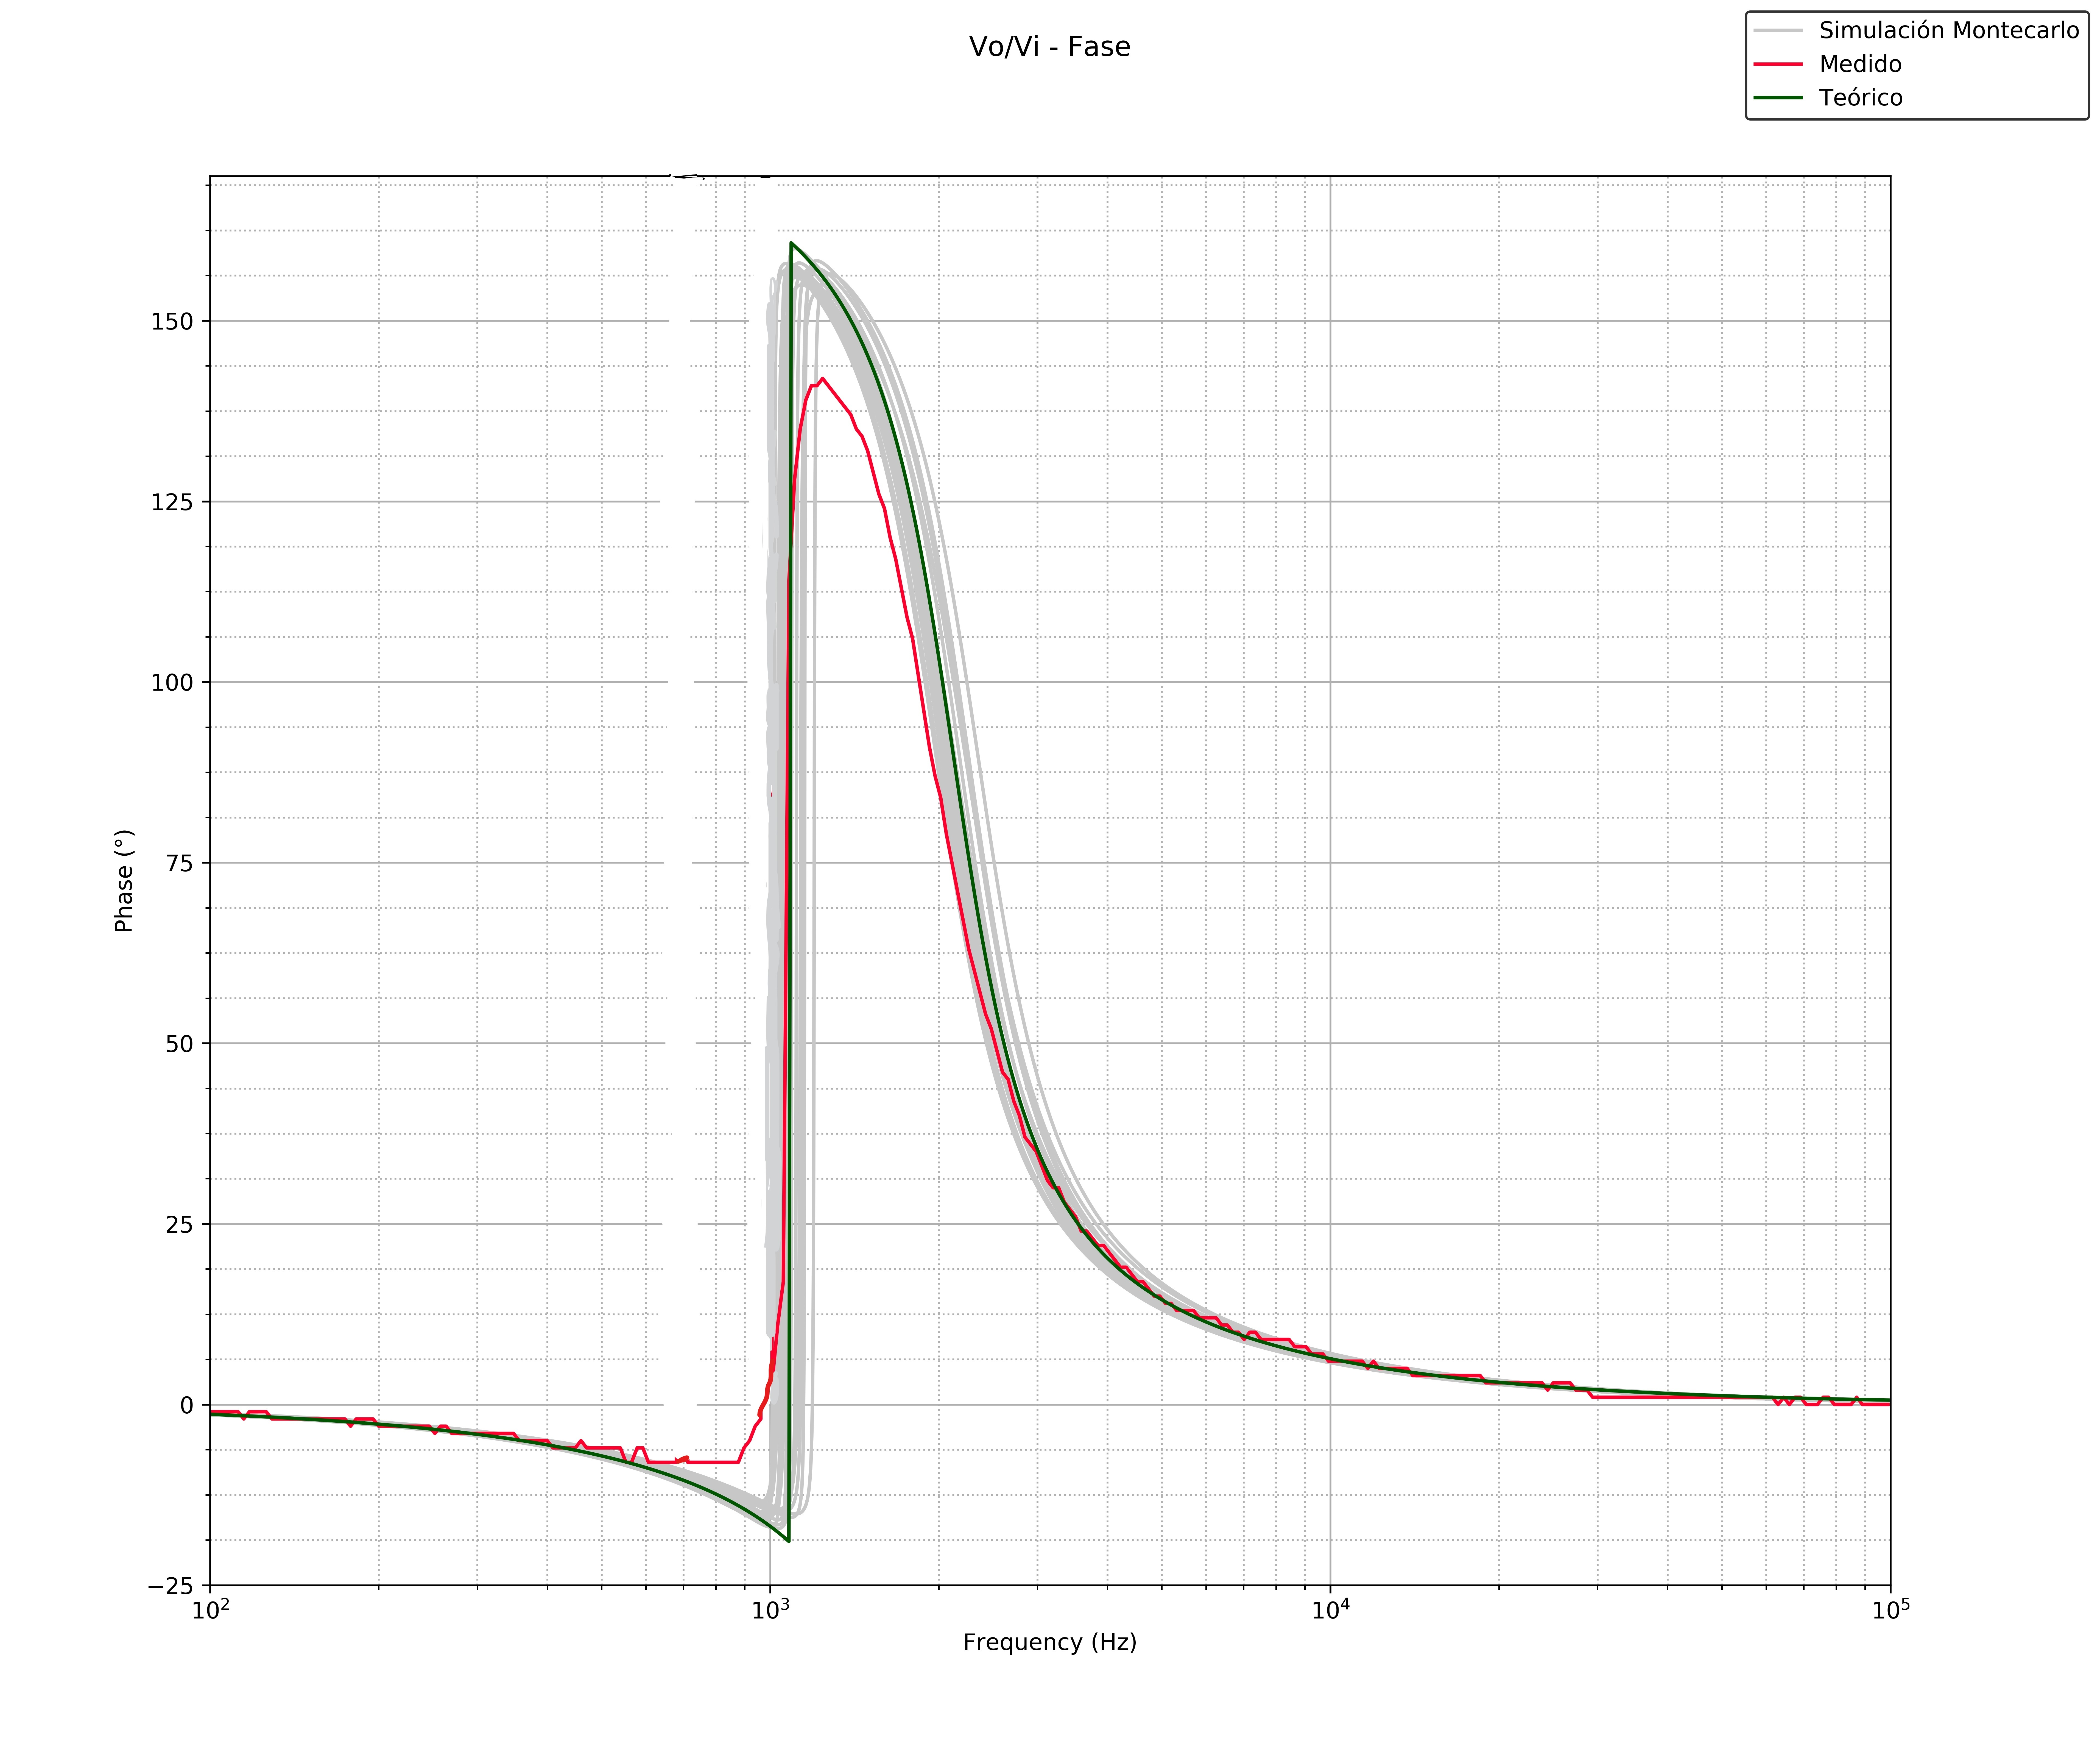
\includegraphics[width=10cm,height=10cm,keepaspectratio]{../EJ1/00GRAFICOS/vovifase.jpg}
	\caption{Fase de la transferencia del circuito.}
	\label{vovi_fase}
\end{figure}

El gr\'afico del m\'odulo de la funci\'on transferencia, figura \ref{vovi_mod}, permite ver que los Q de la medici\'on fueron menores que aquellos de los c\'alculos te\'oricos. Si bien el Q del polo presenta una peque\~na respecto a la especificada te\'oricamente en el dise\~no del circuito, el Q del cero presenta un cambio notable. Te\'oricamente el mismo deb\'a ser infinito, pero en la implementaci\'on eso no ocurre. Sin embargo, la atenuaci\'on no deja de ser considerable.


\subsection{ ''Notch Depth''}

Se llama $notch depht$ a la profundidad del pico del filtro notch. Esta profundidad es la m\'axima atenuaci\'on que presentar\'a la se\~nal de entrada.

\paragraph*{C\'alculo te\'orico}

Observando la funci\'on transferencia ideal del circuito, que se transcribe a continuaci\'on:

\begin{equation}
H(s) = \frac{2}{1+k^2} \cdot \frac{s^2 + \left( \frac{k}{RC}\right)^2}{s^2 + \frac{1}{RCQ} s + \left(\frac{1}{RC}\right)^2}
\label{vovi_simple2}
\end{equation}

Se puede decir que dado que el Q del cero es $\infty$, el pico del notch llega a $-\infty$. Esto es para el caso ideal, el cual no se cumple al momento de medir. Para ver anal\'iticamente lo que ocurre con el pico del notch, a continuaci\'on se presenta la derivada de la transferencia obtenida, luego de haber reemplazado en la expresi\'on de la funci\'on transferencia con los valores de los componentes, se deriva la siguiente expresi\'on:

\begin{equation}
H(s) = 1,59 \cdot \frac{s^2+73,52 \cdot 10^6}{1,26 s^2 + 6666,6 s + 177,78 \cdot 10^6}
\end{equation}

\begin{equation}
H'(s) = \frac{\left(10,6 \cdot 10^3 s^{2} + 33,15 \cdot 10^7 s - 77,93 \cdot 10^{10}\right)}{s^{4} + 13,33 \cdot 10^3 s^{3} + 40 \cdot 10^7 s^{2} + 23,7 \cdot 10^11 s + 3.16 \cdot 10^{16}}
\label{deriv}
\end{equation}

Reemplazando con $s=j\cdot2\cdot \pi \cdot f$:

\begin{equation}
H'(f) = \frac{- 41,85  \cdot 10^4 f^{2} + 2083169982.40241 i f - 779304206880.0}{1558.54545654404 f^{4} - 3307303.10587019 i f^{3} - 15791507409.6255 f^{2} + 14893513515514.0 i f + 3.16057284 \cdot 10^{16}}
\end{equation}

Igualando la expresi\'on a cero, se obtienen sus dos extremos:

\begin{equation}
	\begin{cases}
	
	\end{cases}
\end{equation}

Para obtener el valor de la frecuencia del notch anal\'ticamente se obtuveo que la frecuencia a la cual se encuentra el pico del notch es a 1,082kHz.

\todo{alan}

Por otro lado, empleando el osciloscopio se observ\'o que la frecuencia para la cual la salida es m\'inima es 1,097kHz. Para dicho punto se obtuvo una atenuaci\'on de 35dB, la cual es menor que la predicha con los c\'alculos te\'oricos al no tratarse de un filtro notch ideal.




\subsection{Conclusiones}

